\documentclass[journal]{vgtc}                % final (journal style)
%\documentclass[review,journal]{vgtc}         % review (journal style)
%\documentclass[widereview]{vgtc}             % wide-spaced review
%\documentclass[preprint,journal]{vgtc}       % preprint (journal style)

%% Uncomment one of the lines above depending on where your paper is
%% in the conference process. ``review'' and ``widereview'' are for review
%% submission, ``preprint'' is for pre-publication, and the final version
%% doesn't use a specific qualifier.

%% Please use one of the ``review'' options in combination with the
%% assigned online id (see below) ONLY if your paper uses a double blind
%% review process. Some conferences, like IEEE Vis and InfoVis, have NOT
%% in the past.

%% Please note that the use of figures other than the optional teaser is not permitted on the first page
%% of the journal version.  Figures should begin on the second page and be
%% in CMYK or Grey scale format, otherwise, colour shifting may occur
%% during the printing process.  Papers submitted with figures other than the optional teaser on the
%% first page will be refused. Also, the teaser figure should only have the
%% width of the abstract as the template enforces it.

%% These few lines make a distinction between latex and pdflatex calls and they
%% bring in essential packages for graphics and font handling.
%% Note that due to the \DeclareGraphicsExtensions{} call it is no longer necessary
%% to provide the the path and extension of a graphics file:
%% 
\includegraphics{diamondrule} is completely sufficient.
%%
\ifpdf%                                % if we use pdflatex
  \pdfoutput=1\relax                   % create PDFs from pdfLaTeX
  \pdfcompresslevel=9                  % PDF Compression
  \pdfoptionpdfminorversion=7          % create PDF 1.7
  \ExecuteOptions{pdftex}
  \usepackage{graphicx}                % allow us to embed graphics files
  \DeclareGraphicsExtensions{.pdf,.png,.jpg,.jpeg} % for pdflatex we expect .pdf, .png, or .jpg files
\else%                                 % else we use pure latex
  \ExecuteOptions{dvips}
  \usepackage{graphicx}                % allow us to embed graphics files
  \DeclareGraphicsExtensions{.eps}     % for pure latex we expect eps files
\fi%

%% it is recomended to use ``\autoref{sec:bla}'' instead of ``Fig.~\ref{sec:bla}''
\graphicspath{{figures/}{pictures/}{images/}{./}} % where to search for the images

\usepackage{microtype}                 % use micro-typography (slightly more compact, better to read)
\PassOptionsToPackage{warn}{textcomp}  % to address font issues with \textrightarrow
\usepackage{textcomp}                  % use better special symbols
\usepackage{mathptmx}                  % use matching math font
\usepackage{times}                     % we use Times as the main font
\renewcommand*\ttdefault{txtt}         % a nicer typewriter font
\usepackage{cite}                      % needed to automatically sort the references
\usepackage{tabu}                      % only used for the table example
\usepackage{booktabs}                  % only used for the table example
%% We encourage the use of mathptmx for consistent usage of times font
%% throughout the proceedings. However, if you encounter conflicts
%% with other math-related packages, you may want to disable it.

%% In preprint mode you may define your own headline.
%\preprinttext{To appear in IEEE Transactions on Visualization and Computer Graphics.}

%% If you are submitting a paper to a conference for review with a double
%% blind reviewing process, please replace the value ``0'' below with your
%% OnlineID. Otherwise, you may safely leave it at ``0''.
\onlineid{0}

%% declare the category of your paper, only shown in review mode
\vgtccategory{Research}
%% please declare the paper type of your paper to help reviewers, only shown in review mode
%% choices:
%% * algorithm/technique
%% * application/design study
%% * evaluation
%% * system
%% * theory/model
\vgtcpapertype{please specify}

%% Paper title.
\title{Visualization of Reported UFO Sightings}

%% This is how authors are specified in the journal style

%% indicate IEEE Member or Student Member in form indicated below
\author{Peter Bernstein, Emily Dutile, Abigail Skelton, and Lydia Zakynthinou}
\authorfooter{
%% insert punctuation at end of each item
\item
Emily Dutile and Abigail Skelton are graduate students at Northeastern University. E-mail: \{dutile.e, skelton.a\}@husky.neu.edu.
\item
Peter Bernstein and Lydia Zakynthinou are PhD students at Northeastern University. E-mail: \{bernstein.p, zakynthinou.l\}@husky.neu.edu.
}


%other entries to be set up for journal
\shortauthortitle{Biv \MakeLowercase{\textit{et al.}}: Visualization of Reported UFO Sightings}
%\shortauthortitle{Firstauthor \MakeLowercase{\textit{et al.}}: Paper Title}

%% Abstract section.
\abstract{Reports of unidentified flying objects (\textit{UFOs}) have sparked amateur research, government investigations,
 and large popular interest in the last five decades. Most reported UFOs are later identified as natural phenomena or
 conventional objects. However, there is a considerable body of reports about objects that are not identified, which are 
 often rumored as claims of observations of
 extraterrestrial crafts, raising questions about life on other planets and
 extraterrestrials visiting Earth. Scientists in their majority have naturally greeted the topic with
 skepticism but it widely recognized that answering these questions would be of great
 importance and a step towards understanding the universe. We provide an interactive
 visualization of the reported UFO sightings in the United States in the period of 1964-2017,
 aiming to help any interested user explore these sightings.
} % end of abstract

%% Keywords that describe your work. Will show as 'Index Terms' in journal
%% please capitalize first letter and insert punctuation after last keyword
\keywords{Visualization, Map, Interactivity, Unidentified Flying Object, UFO, United States.}

%% ACM Computing Classification System (CCS). 
%% See <http://www.acm.org/class/1998/> for details.
%% The ``\CCScat'' command takes four arguments.

\CCScatlist{ % not used in journal version
 \CCScat{K.6.1}{Management of Computing and Information Systems}%
{Project and People Management}{Life Cycle};
 \CCScat{K.7.m}{The Computing Profession}{Miscellaneous}{Ethics}
}

%% Uncomment below to include a teaser figure.
\teaser{
  \centering
  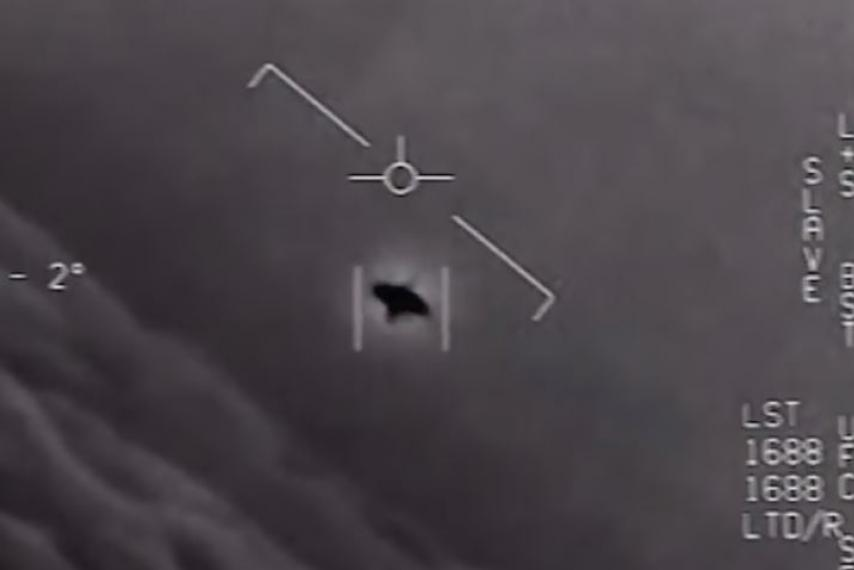
\includegraphics[width=\linewidth]{ufoimage}
  \caption{UFOs are ``proved beyond reasonable doubt"��: A rotating ``��glowing aura"� traveling at high speeds that was captured from a Navy F/A-18 Super Hornet. \cite{pentagon}}
	\label{fig:teaser}
}

%% Uncomment below to disable the manuscript note
\renewcommand{\manuscriptnotetxt}{}

%% Copyright space is enabled by default as required by guidelines.
%% It is disabled by the 'review' option or via the following command:
%\nocopyrightspace

\vgtcinsertpkg

%%%%%%%%%%%%%%%%%%%%%%%%%%%%%%%%%%%%%%%%%%%%%%%%%%%%%%%%%%%%%%%%
%%%%%%%%%%%%%%%%%%%%%% START OF THE PAPER %%%%%%%%%%%%%%%%%%%%%%
%%%%%%%%%%%%%%%%%%%%%%%%%%%%%%%%%%%%%%%%%%%%%%%%%%%%%%%%%%%%%%%%%

\begin{document}

%% The ``\maketitle'' command must be the first command after the
%% ``\begin{document}'' command. It prepares and prints the title block.

%% the only exception to this rule is the \firstsection command
\firstsection{Introduction}

\maketitle

%% \section{Introduction} %for journal use above \firstsection{..} instead
An unidentified flying object (UFO) is a perceived object in the sky that is not readily identified. The term UFO (initially, \textit{UFOB}) appeared in 1953 when the United States Air Force used it to describe ``any airborne object which by performance, aerodynamic characteristics, or unusual features, does not conform to any presently known aircraft or missile type, or which cannot be positively identified as a familiar object" \cite{ufowiki}. Since the 1950s, UFOs have become a major subject of interest in the popular culture and an inspiration for several movies and books \cite{history}. The reason for this is the fact that UFOs are linked to rumored extraterrestrial aircrafts, and if this were true it would suggest that extraterrestrials have visited our planet.\\
\indent Although UFOs are largely connected to this theme, it is true that for most of the reported cases the objects are identified to be ordinary or to be caused by natural phenomena after careful investigation. Most commonly, UFOs are identified to actually be astronomical objects, aircrafts, balloons (e.g. weather, research balloons), atmospheric or light phenomena (e.g. clouds, mirages), other atmospheric objects (e.g. birds), or, in some rare cases, hoaxes. The percentage of reports of objects that remain unidentified lies between 5\% and 20\%  \cite{ufowiki}. However, this is a large enough percentage to spur a significant amount of government research and funds as well as scientific attention.\\
\indent Of the most recently revealed government programs on UFOs is the U.S. Defense Department's \textit{Advanced Aerospace Threat Identification Program} \cite{pentagon}. The program, which was led by military intelligence official Luis Elizondo, investigated evidence of UFOs and extraterrestrial life from 2007 to 2012, with an annual budget of 22 million dollars. In 2012 it was shuttered due to a change in the department's funding priorities, but Elizondo oversaw UFO investigations until this past October. He is convinced that this is a matter of importance and even contends that UFOs are ``proved beyond reasonable doubt" (Fig.1). As for the scientific community, the recent \textit{Breakthrough Listen Program} \cite{listen}, located in the Astronomy Department of the University of California, Berkeley, is the most scientifically comprehensive search for intelligent extraterrestrial communications in the Universe to date \cite{listenwiki}. It counts 100 million dollars in funding and it became more publicly known due to the statements of renowned physicist Stephen Hawking on alien life and his support of the program \cite{hawking}.

It is clear that the subject is controversial but, at the same time, most would agree that it requires research and attention. Therefore, it is important that there is a general awareness of the subject to the public. To this end, we created an interactive web-based visualization that allows the user to explore reports of sightings in the United States. It is intended to be pleasing and to give an overview of the reported sightings in the United States throughout the years, as well as the ability to drill down in order to explore characteristics of more specific areas and sightings.

The data we are using is posted on the website of the National UFO Report Center, whose head is Peter Davenport. The Center's website provides an online form as well as a hotline for reports of UFO sightings and these reports are annotated by Peter Davenport himself before they are posted in the database. Each report includes the date and time of the sighting, its duration, shape, location, and description summary (possibly including notes of Peter Davenport in double parentheses), as well as the date the report was posted.

\begin{table}[h]
\caption{Data attributes} % title name of the table
\centering % centering table
\begin{tabular}{c c c} % creating 3 columns
\hline\hline % inserting double-line
 Term & Type of Variable & Example\\ [0.5ex]
\hline % inserts single-line

Date & quantitative & 1/12/10 21:30\\[1ex] %space

City & categorical & Fairbanks\\[1ex] %space

State & categorical & AK\\[1ex] %space

Shape & categorical	& Disk\\[1ex] %space

Duration & quantitative & about 1.5 minutes\\[1ex] %space

Summary & & ``We saw..."\\[1ex] %space

Date Posted & quantitative & 1/12/2012\\[1ex] %space

\hline 
\end{tabular}
\label{tab:PPer}
\end{table}

\section{Related Works}

\textbf{Visualizations of the UFO dataset:}
The dataset we are using has been popular on Kaggle which led two data visualization experts, Pooja Gandhi and Adam Crahen, to use it in their DuoDare project on their DataDuo blog \cite{dataduo}. The DuoDare was a project where each month one of the two experts would choose a dataset and call the other on a battle for the best visualization. The two visualizations that the experts came up with for this dataset included, among others, interactive maps, area charts, bar charts, and calendar heat-maps. Both visualizations as well as our own include a map of the United States. In Pooja Ghandi's visualization a point on the map corresponds to an area and hovering over the point shows a moving tooltip of the number of sightings that have been reported in that area. In Adam Crahen's visualization each point corresponds to a single sighting and hovering over the point shows the details of the sighting. Adam Crahen's visualization includes a calendar heat-map, which also allows the user to click on a particular year/month/weekday/hour and filter the sightings she sees. Pooja Ghandi's visualization includes an area chart of the number of sightings through the years and allows the user to filter the data over time by hovering over a particular vertical line on the area chart. This action also updates a donut chart showing the number of sightings in that year as a percentage over the total number of sightings. In addition to these, it includes two horizontal bar charts showing the five locations/shapes with the highest number of sightings, as well as two visualizations regarding the top five countries besides the United States with the highest number of sightings. 

In our visualization we use the same encoding as Adam Crahen for the overview task, i.e. we use a map where each point corresponds to a sighting. However, instead of showing a static map of all the points, we populate the map over time. The user can pause this procedure by clicking on the time-slider. This allows her to explore more patterns about the way the sightings occur over the years, on top of giving an overall picture of the sightings, whereas the other two visualizations only use filtering to allow the user to explore these patterns. As an extra overview feature, we color each state based on the number of sightings that have occurred in that state. In addition, our visualization is different from the other two since it also supports drilling down in the data. It allows the user to choose a particular state to see the sightings of that state in more detail and it shows a line chart of the number of sightings of the state over time (instead of the area chart Pooja Gandhi used for a similar task). Finally, it allows the user to brush over an area in the state, thus selecting a group of sightings, and it updates the line chart of the sightings over time based on these sightings only. We believe that this additional exploration based on the state and area is more intriguing and would make the visualization more interesting and enjoyable to the user. We base this on the fact that our visualization supports the task of ``What sightings have happened in my area?" which is a common question when thinking about this subject.

\textbf{Visualizing geographic spatial data:}
Since we have geographic spatial data, we chose a map to represent them. There are several types of maps, based on the type of surface the Earth is projected on. There are three main types of projections: cylindrical, conical, and azimuthal \cite{projections}. Although cylindrical projections incur a significant amount of distortion (\cite{distortion}), the Mercator map, which corresponds to a cylindrical projection, is the most popular type of map. Since it is more important that the user is familiar with what they are seeing than deriving exact conclusions on the data, we chose to use the Mercator map.

\section{Process}
In this section we focus on the necessary steps that we took successfully create our project. Most of the steps were prescribed for us beforehand as requirements for the final project for our data visualization course. \\

\textbf{Initial data selection:} With requirements for a class project already available to us, this dataset became appealing to us for its cleanliness and public availability. The key requirements were that we make an interactive, web-based visualization with at least two different visual encodings and two features from brushing and linking, overview, and details-on-demand. The existing visualizations of this data we found \cite{dataduo} left the option to incorporate brushing and linking of time with the spacial data as well as a few other features as a novel direction to head in. We found the whole subject to be amusing and felt a broad audience would be able to have fun exploring an interactive visualization of these data.

\textbf{Interview with field expert:} Having decided to use the the National UFO Report Center's dataset for our project, we conducted a phone interview with its head, Peter Davenport to help us understand his website and dataset better. The current iteration of the website was set up in 1995 and hosts approximately 145,000 alleged sightings, with a noticeable uptick since the option to report a sighting via the internet became available. Currently there is a weekly UFO update on Coast to Coast AM radio and the website boasts many details with images of suspected sightings, however no visualizations of the dataset as a whole. After this interview we were able to decide which tasks were most important for us to satisfy in our visualization (see 3.1).

\textbf{Prototyping workflows based on feedback:} Based on the tasks outlined in 3.1, we each created different sketches that we discussed extensively with each other as well as with the teaching staff before incorporating the best features of those sketches into a final workflow to keep as a goal.  Further along the way, there was an interactive feature testing session where we tested a basic D3 prototype of our visualization with our classmates. The feedback we gathered served to help us tailor the design to users less familiar than ourselves with the tool and the data behind it.% (ex: a new color scheme to be more colorblind-friendly, or whatever feedback we get).

%\begin{itemize}
%\item We interviewed Peter Davenport, the director of the National UFO Reporting Center to help us understand our dataset better.
%\item We decided on what the important tasks are for our visualization (see 3.1).
%\item We came up with different sketches to support these tasks.
%\item We discussed all our ideas and concluded on the visualization we wanted to implement. 
%\item We will provide users (our classmates) with a basic D3 interactive prototype of our visualization and get their feedback.
%\item We will finish up our visualization based on our user feedback.
%\end{itemize}

\subsection{Task Analysis}
The domain tasks our visualization supports are in Table 2.


\begin{table}[h]
\caption{Domain Tasks} % title name of the table
\centering % centering table
\begin{tabular}{c c c} % creating 3 columns
\hline\hline % inserting double-line
 Task & Abstraction\\ [0.5ex]
\hline % inserts single-line

Observe how the UFO \\sightings occur throughout the years & Present\\[1ex] %space

Observe all UFO sightings of a particular year \\ and specific details (such as shape) & Discover\\[1ex] %space

Curiosity stimulation & Enjoy\\[1ex] %space

Look for areas with high number of sightings & Search/Explore\\[1ex] %space

Are there clusters of UFO\\ sightings according to geographic area? & Cluster\\[1ex] %space

Learn details of sighting & Retrieve Value\\[1ex] %space

When did the sightings of a particular area \\(e.g. my hometown) occur? & Filter\\[1ex] %space

What state has the most sightings? & Find Extremum\\[1ex] %space

What date has the most sightings? & Find Extremum\\[1ex] %space

\hline 
\end{tabular}
\label{tab:PPer}
\end{table}


In general these tasks can be categorized into two abstract tasks.
\begin{itemize}
\item \textbf{(T1)} Overview task:
\item \textbf{(T2)} Drill-Down task:
\end{itemize}

\section{Design}
For the abstract tasks, we chose the following visualization idioms (Table 3).


\begin{table}[h]
\caption{Visualizing the Abstract Tasks} % title name of the table
\centering % centering table
\begin{tabular}{c c c} % creating 3 columns
\hline\hline % inserting double-line
 Abstract Task & Visualization Idiom\\ [0.5ex]
\hline % inserts single-line

Overview & Map\\[1ex] %space

Drill-Down & Map and Line Chart\\[1ex] %space

\hline 
\end{tabular}
\label{tab:PPer}
\end{table}

\textbf{Visual Encoding and Interaction Choices:}

\begin{itemize}

\item Points on map for representation of geographic data
\item Sequential color scale for frequency of sightings on choropleth map
\item Retrieve details of sighting on tooltip on hover
\item Clicking on state to change the drilled-down view (hovering only affects tooltip)
\item Line chart for frequency of sightings of state over time (position as a channel for quantitative value)
\item Brush to choose sightings of an area for which the user wants to know information about when they occurred

\end{itemize}

\textbf{Implementation:}


\section{Discussion}
\subsection{Reflections?}
\subsection{Future Work}
This paper focused on the UFO data we worked with, the tasks we sought to implement, and the visualization design that resulted from these requirements as well as through acquired feedback. There are many features we would like to be able to include in the future, however. Among the most interesting would be to associate historical weather data with the dates of the alleged UFO sightings. Additionally, plotting sources of red flags such as airports or weather balloons would be of use in explaining a large number of sightings. The biggest challenge at the moment is acquiring a suitable dataset containing this information in a reasonable format. 


\section{Conclusion}
We created a web-based interactive visualization providing a novel view of data originally gathered by the National UFO Report Center of thousands of alleged UFO sightings around the country. We incorporated interactivity tools such as brushing and linking to make it easier to dynamically view reported sightings on a United States map and select only reports within years ranges of interest. This allows a map to be less cluttered than existing maps and thus also allows for details-on-demand to be easier to use as there is less ambiguity of where a user is pointing. We use an appealing color palate for the task at hand and create an environment that is amusing and engaging to users interested in understanding the scale of belief in conspiracies or UFOs.




\begin{thebibliography}{9}

\bibitem{blocks} 
Mike Bostock.
\textit{Blocks}. 
Click-to-Zoom via Transform,
\\\url{https://bl.ocks.org/mbostock/2206590}

\bibitem{ufoimage} 
Newsweek.
\textit{UFO existence proven beyond reasonable doubt says former head of Pentagon alien program}.
\\\url{http://www.newsweek.com/ufo-existence-proven-beyond\\-reasonable-doubt-says-former-head-pentagon-alien-758293}

\bibitem{dataduo}
DataDuo - DuoDare Project on UFO sightings
\\\url{https://thedataduo.com/2017/11/11/duodare-3\\-ufo-sightings/}

\bibitem{ufowiki}
Wikipedia.
\textit{Unidentified flying object}.
\\\url{https://wikipedia.org/wiki/Unidentified\_flying\_object}

\bibitem{history}
History.
\textit{History of UFOs}.
\\\url{https://www.history.com/topics/history-of-ufos}

\bibitem{pentagon}
The Guardian.
\textit{Pentagon admits running secret UFO investigation for five years}.
\\\url{https://www.theguardian.com/world/2017/dec/17/\\pentagon-admits-running-secret-ufo-investigation-for-five-years}

\bibitem{listen}
The Guardian.
\textit{Why we keep scanning the skies for signs of alien intelligence}.
\\\url{https://www.theguardian.com/science/2017/dec/22/\\why-we-keep-scanning-the-skies-for-signs-of-alien-intelligence}

\bibitem{listenwiki}
Wikipedia.
\textit{Breakthrough Listen}.
\\\url{https://en.wikipedia.org/wiki/Breakthrough\_Listen}

\bibitem{hawking}
Newsweek.
\textit{Stephen Hawking on alien life, extraterrestrials and the possibility of UFOs visiting Earth}.
\\\url{http://www.newsweek.com/stephen-hawking-death-alien\\-contact-aliens-theory-ufo-search-breakthrough-844920}

\bibitem{projections}
Geokov.
\textit{Map Projections - Types and Distortion Patterns}
\\\url{http://geokov.com/education/map-projection.aspx}

\bibitem{distortion}
Mike Bostock.
Map Projection Distortions
\\\url{https://bl.ocks.org/mbostock/3709000}

\end{thebibliography}





%% if specified like this the section will be committed in review mode


%\bibliographystyle{abbrv}
\bibliographystyle{abbrv-doi}
%\bibliographystyle{abbrv-doi-narrow}
%\bibliographystyle{abbrv-doi-hyperref}
%\bibliographystyle{abbrv-doi-hyperref-narrow}

\bibliography{template}
\end{document}

